\begin{center}
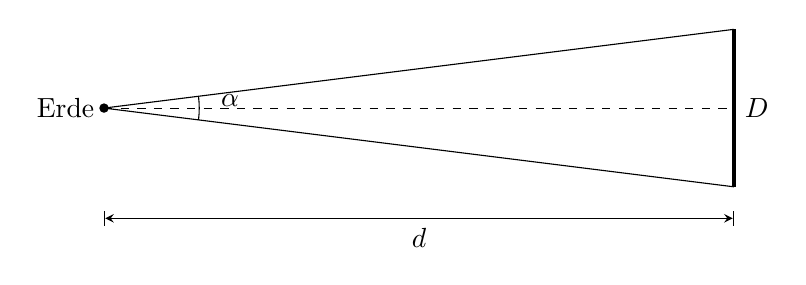
\begin{tikzpicture}[>=stealth]
 \fill (0,0) circle (0.06) node[left] {Erde};
 \draw (0,0) -- (8,1);
 \draw (0,0) -- (8,-1);
 \draw[very thick] (8,-1) -- (8,1) node[midway, right] {$D$};
 \draw[dashed] (0,0) -- (8,0);
 \draw (1.2,-0.15) arc (-7.1:7.1:1.2);
 \node at (1.6,0.1) {$\alpha$};
 \draw[|<->|] (0,-1.4) -- (8,-1.4) node[midway, below] {$d$};
\end{tikzpicture}
\end{center}

Nach FoTaBe S.~216 hat die Grosse Magellan'sche Wolke den Durchmesser $D = \DMaO$ und die Entfernung $d = \dMaO$. Die halbe Wolke erscheint unter dem Winkel $\alpha/2$ mit $\tan\frac{\alpha}{2} = \frac{D/2}{d}$, also
\begin{align}
 \alpha &= \alMF \\
   &= 2\arctan\frac{\DMa}{2\cdot\dMa} \\
   &= \alM \approx \result{\alMP{0}{2}}
\end{align}
Das ist rund zwanzigmal so viel wie der Durchmesser des Vollmondes.
